\section{Dockerを使用した深層学習アプリケーションのデプロイ(Ollamaを例に)}
Ollamaは,多様なオープンソースの大規模言語モデル(LLM, Large Language Model)を提供するプラットフォームであり,ユーザーは必要なモデルを検索,ダウンロード,実行できる.また,Open WebUIは,拡張性が高く,ユーザーフレンドリーな自己ホスティング型AIプラットフォームであり,完全オフラインで動作可能.本システムは,OllamaやOpenAI互換APIを含む様々なLLM環境をサポートし,検索拡張生成(Retrieval-Augmented Generation, RAG)用の推論エンジンを内蔵している.これは強力なLLMアプリケーションのデプロイソリューションとなる.

\subsection{NVIDIA Container Toolkitのインストール}
新規インストールされたDockerでは,NVIDIAのCUDAデバイスを直接利用できない.しかし,多くの深層学習およびAIアプリケーションでは,CUDAランタイムライブラリおよびデバイスが必要.そのため,\texttt{NVIDIA Container Toolkit}をインストールする必要がある.

まず,NVIDIAドライバが正常にインストールされているか確認する:
\begin{lstlisting}[language=bash]
nvidia-smi
\end{lstlisting}

次に,\texttt{NVIDIA Container Toolkit}をインストールする:
\begin{lstlisting}[language=bash]
# NVIDIA公式GPGキーを追加
curl -fsSL https://nvidia.github.io/libnvidia-container/gpgkey | sudo gpg --dearmor -o /usr/share/keyrings/nvidia-container-toolkit-keyring.gpg \
  && curl -s -L https://nvidia.github.io/libnvidia-container/stable/deb/nvidia-container-toolkit.list | \
    sed 's#deb https://#deb [signed-by=/usr/share/keyrings/nvidia-container-toolkit-keyring.gpg] https://#g' | \
    sudo tee /etc/apt/sources.list.d/nvidia-container-toolkit.list

# nvidia-container-toolkitのインストール
sudo apt-get update
sudo apt-get install nvidia-container-toolkit
\end{lstlisting}

\subsection{OllamaとOpen WebUIのDockerイメージを使用したデプロイ}
Open WebUIはOllamaと統合されたDockerイメージを提供しており,簡単にデプロイできる.

以下のコマンドを実行:
\begin{lstlisting}[language=bash]
docker run -d --gpus=all \
  -p 11919:8080 \
  -v ollama:[your path]/ollama-model \
  -v open-webui:[your path]/openwebui-data \
  --name open-webui-ollama \
  --restart always \
  ghcr.io/open-webui/open-webui:ollama
\end{lstlisting}

パラメータの説明:
\begin{itemize}
  \item \texttt{run}: コンテナを実行.
  
  \item \texttt{-d}: バックグラウンドで実行.サービス指向型アプリケーションに推奨.
  
  \item \texttt{--gpus=all}: 全てのGPUアクセスを許可.GPUを使用する場合に必要.
  
  \item \texttt{-p 11919:8080}: ポートのマッピング.安全のため,一般的なポート(80と8080など)を避ける.
  
  \item \texttt{-v ollama:/root/.ollama}: モデルの永続化.\\ \texttt{/var/lib/docker/volumes/ollama\_data}にデータを保存.
  
  \item \texttt{-v open-webui:/app/backend/data}: ユーザーデータの永続化.会話履歴やカスタム設定を保存.
  
  \item \texttt{--restart always}: コンテナの自動再起動の設定.コンテナ障害時に復旧する.
  
  \item \texttt{ghcr.io/open-webui/open-webui:ollama}: 使用するイメージを指定.信頼できるソースの使用を推奨.
\end{itemize}

コンテナが正常に起動すると,\texttt{http://localhost:11919} にアクセスできる:

\begin{figure}[H]
    \centering
    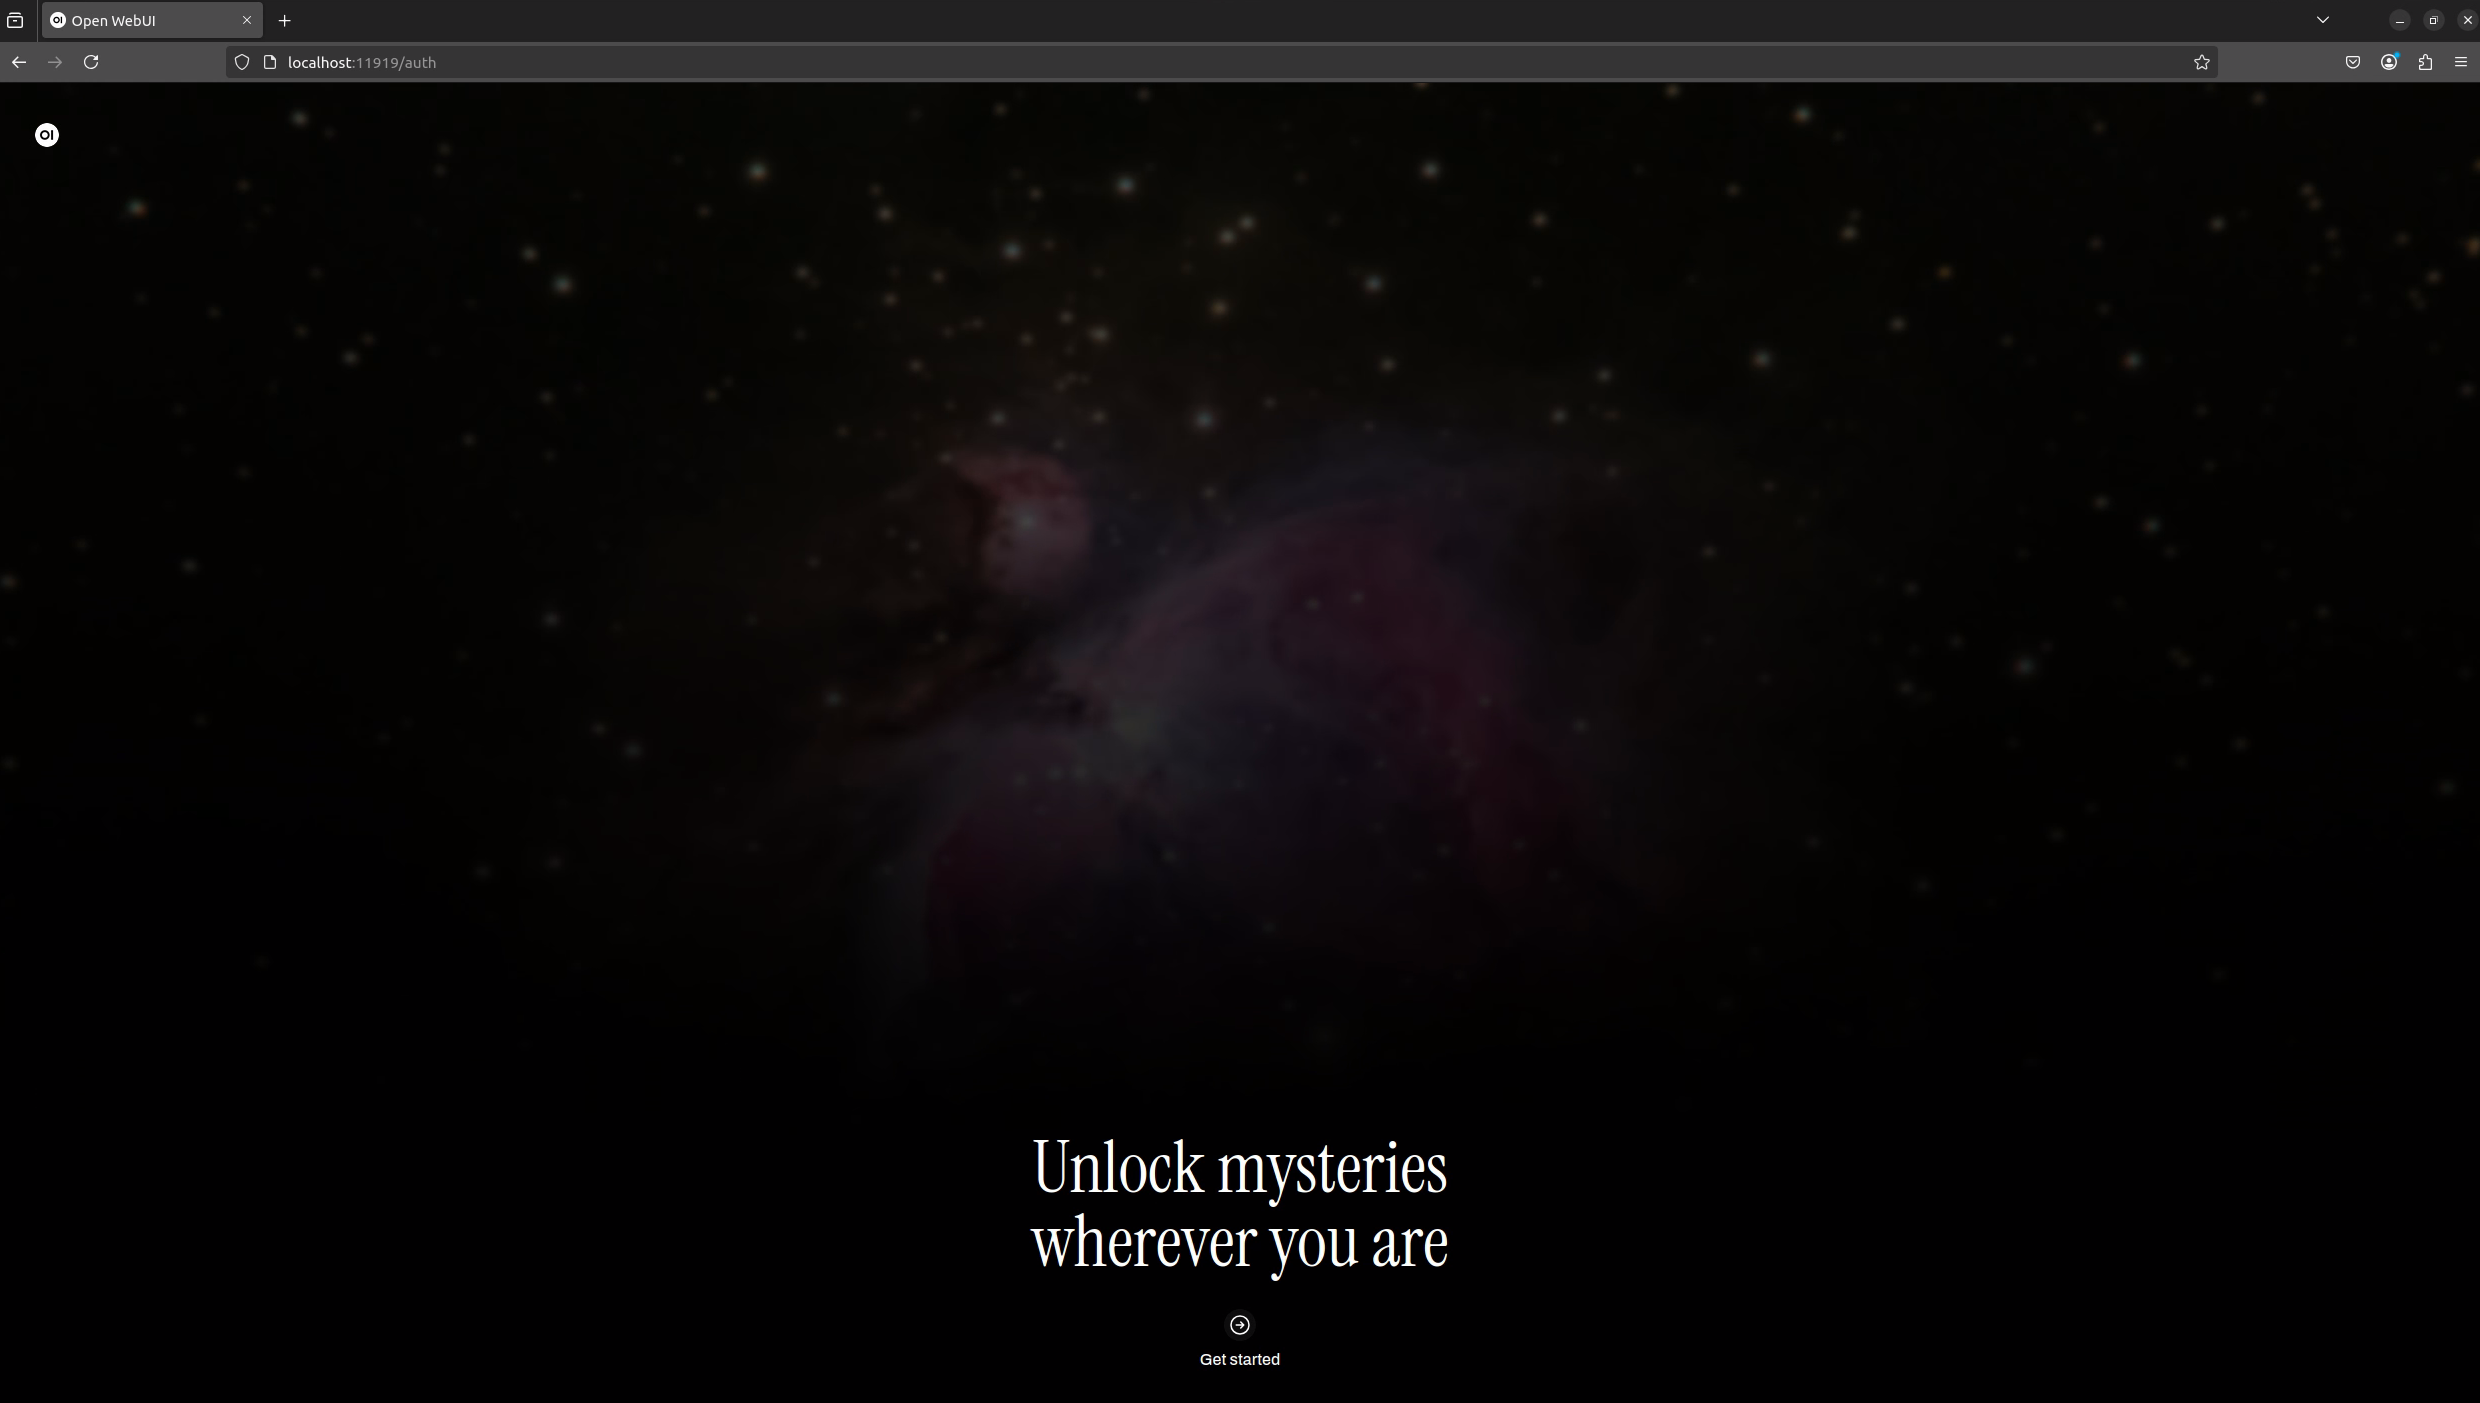
\includegraphics[width=0.8\linewidth]{images/Pasted image 20250304171521.png}
    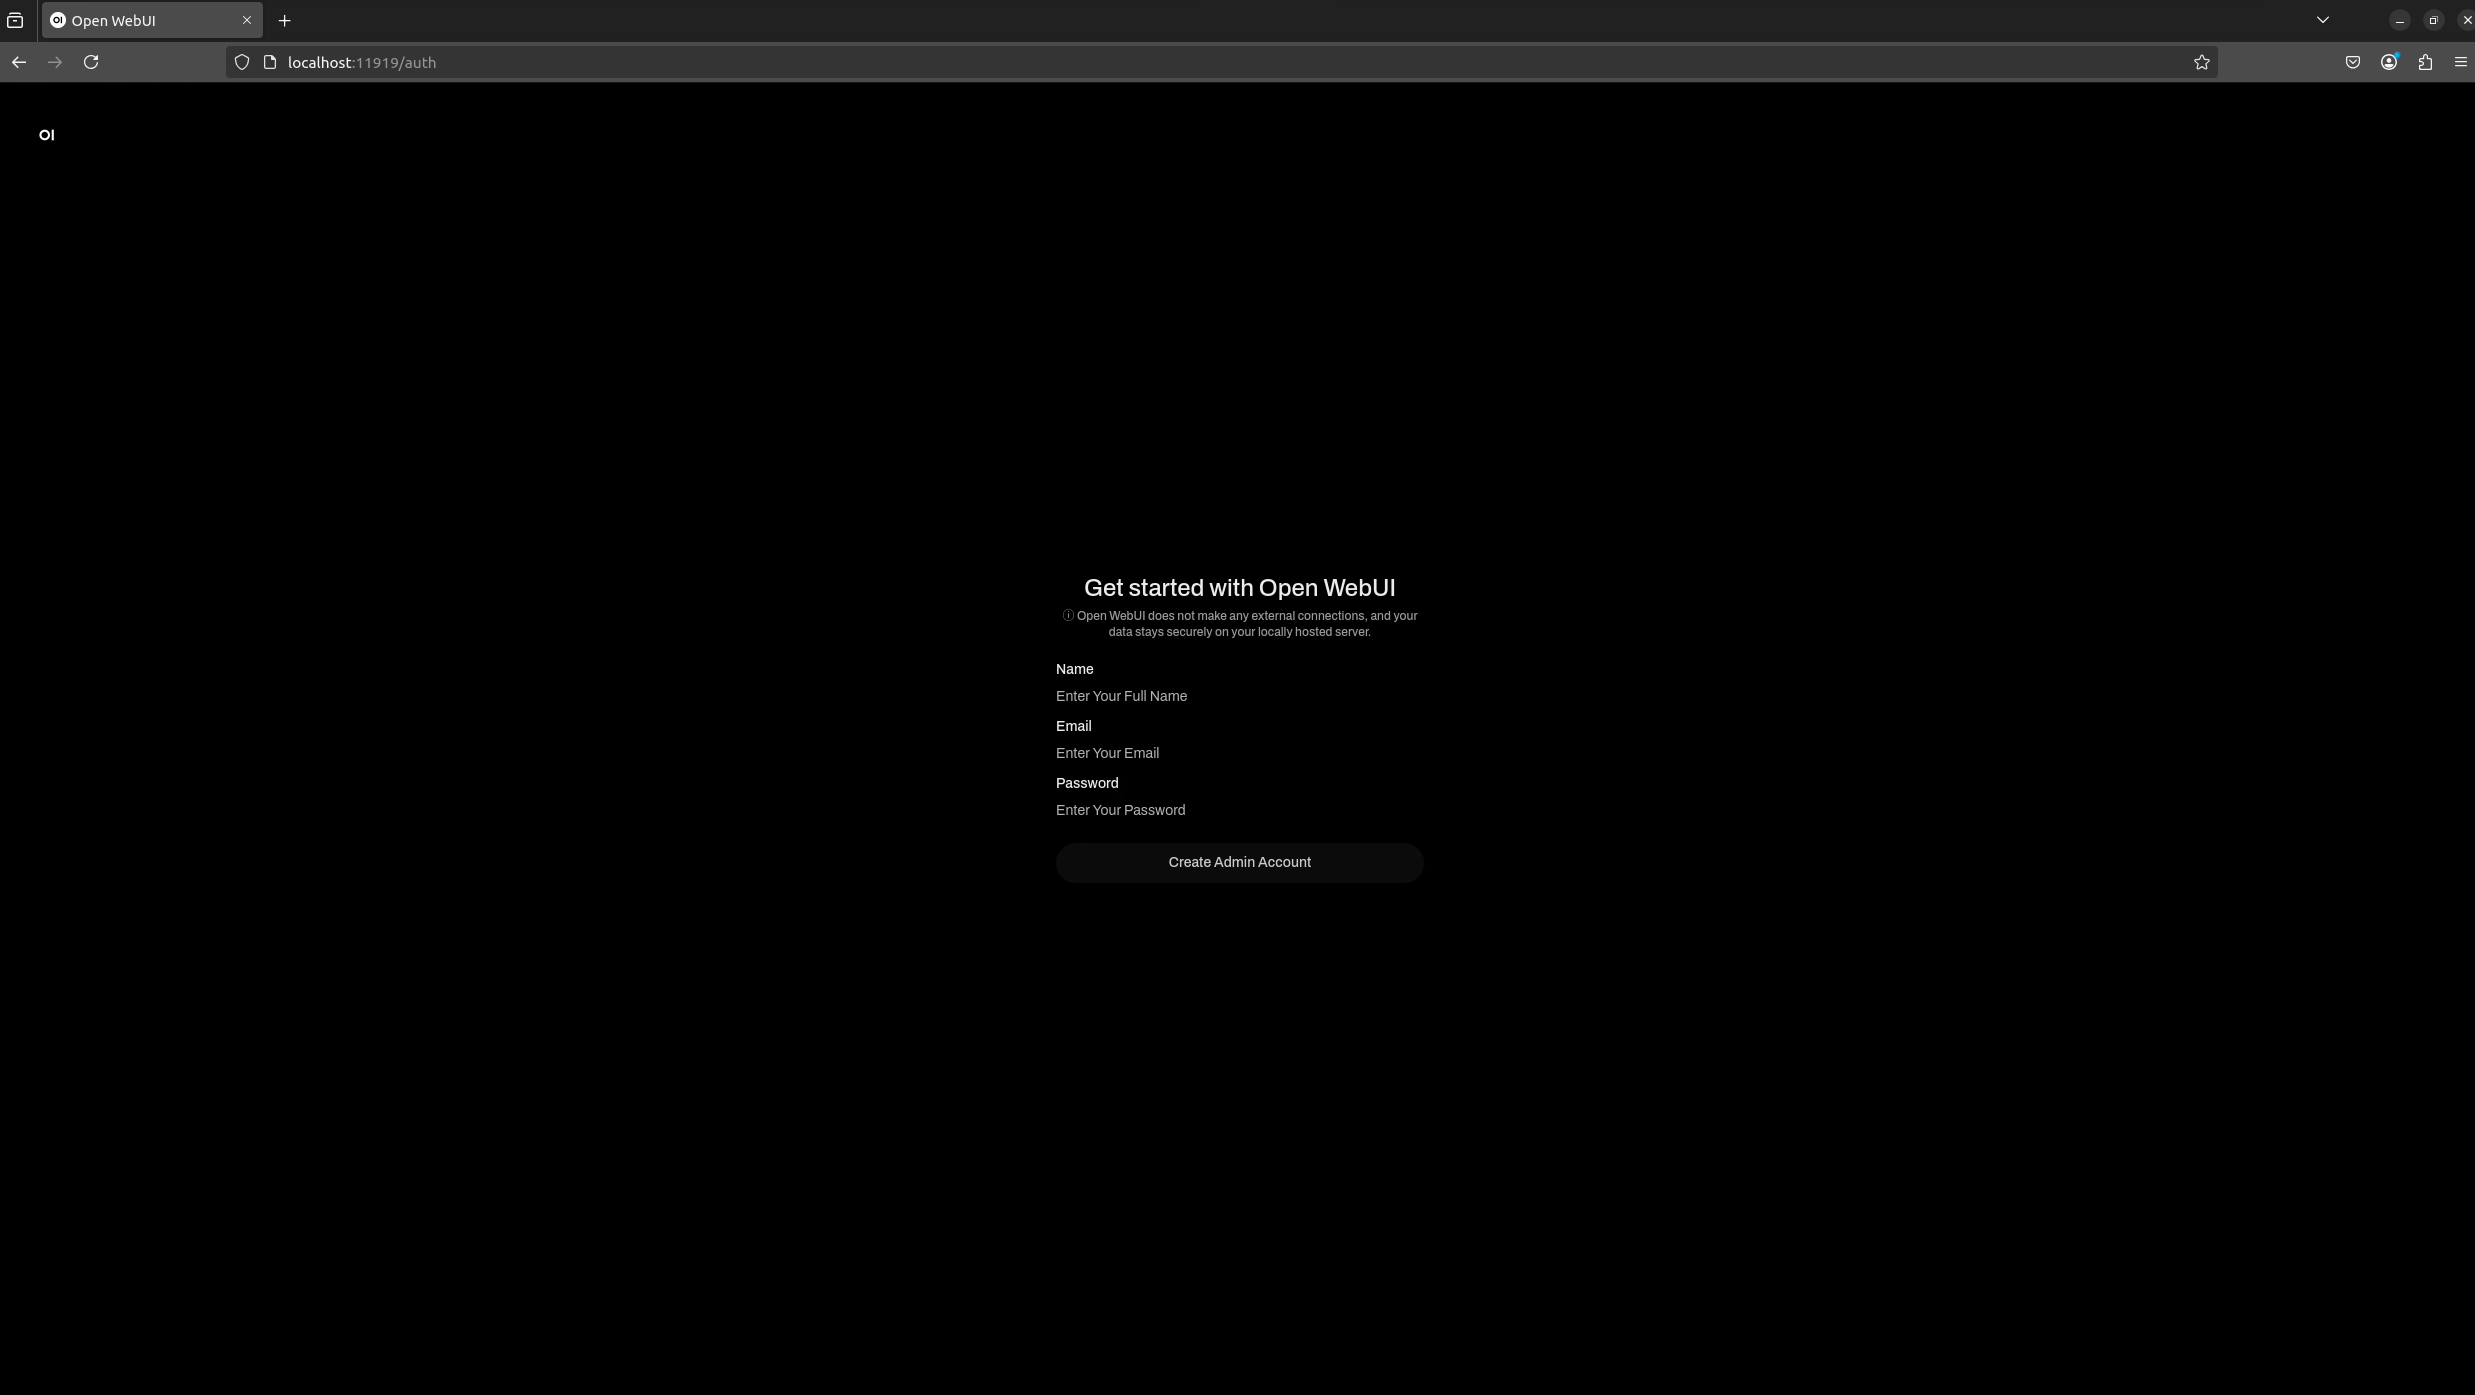
\includegraphics[width=0.8\linewidth]{images/Pasted image 20250304171548.png}
\end{figure}

ログインすると,以下の画面が表示される:
\begin{figure}[H]
    \centering
    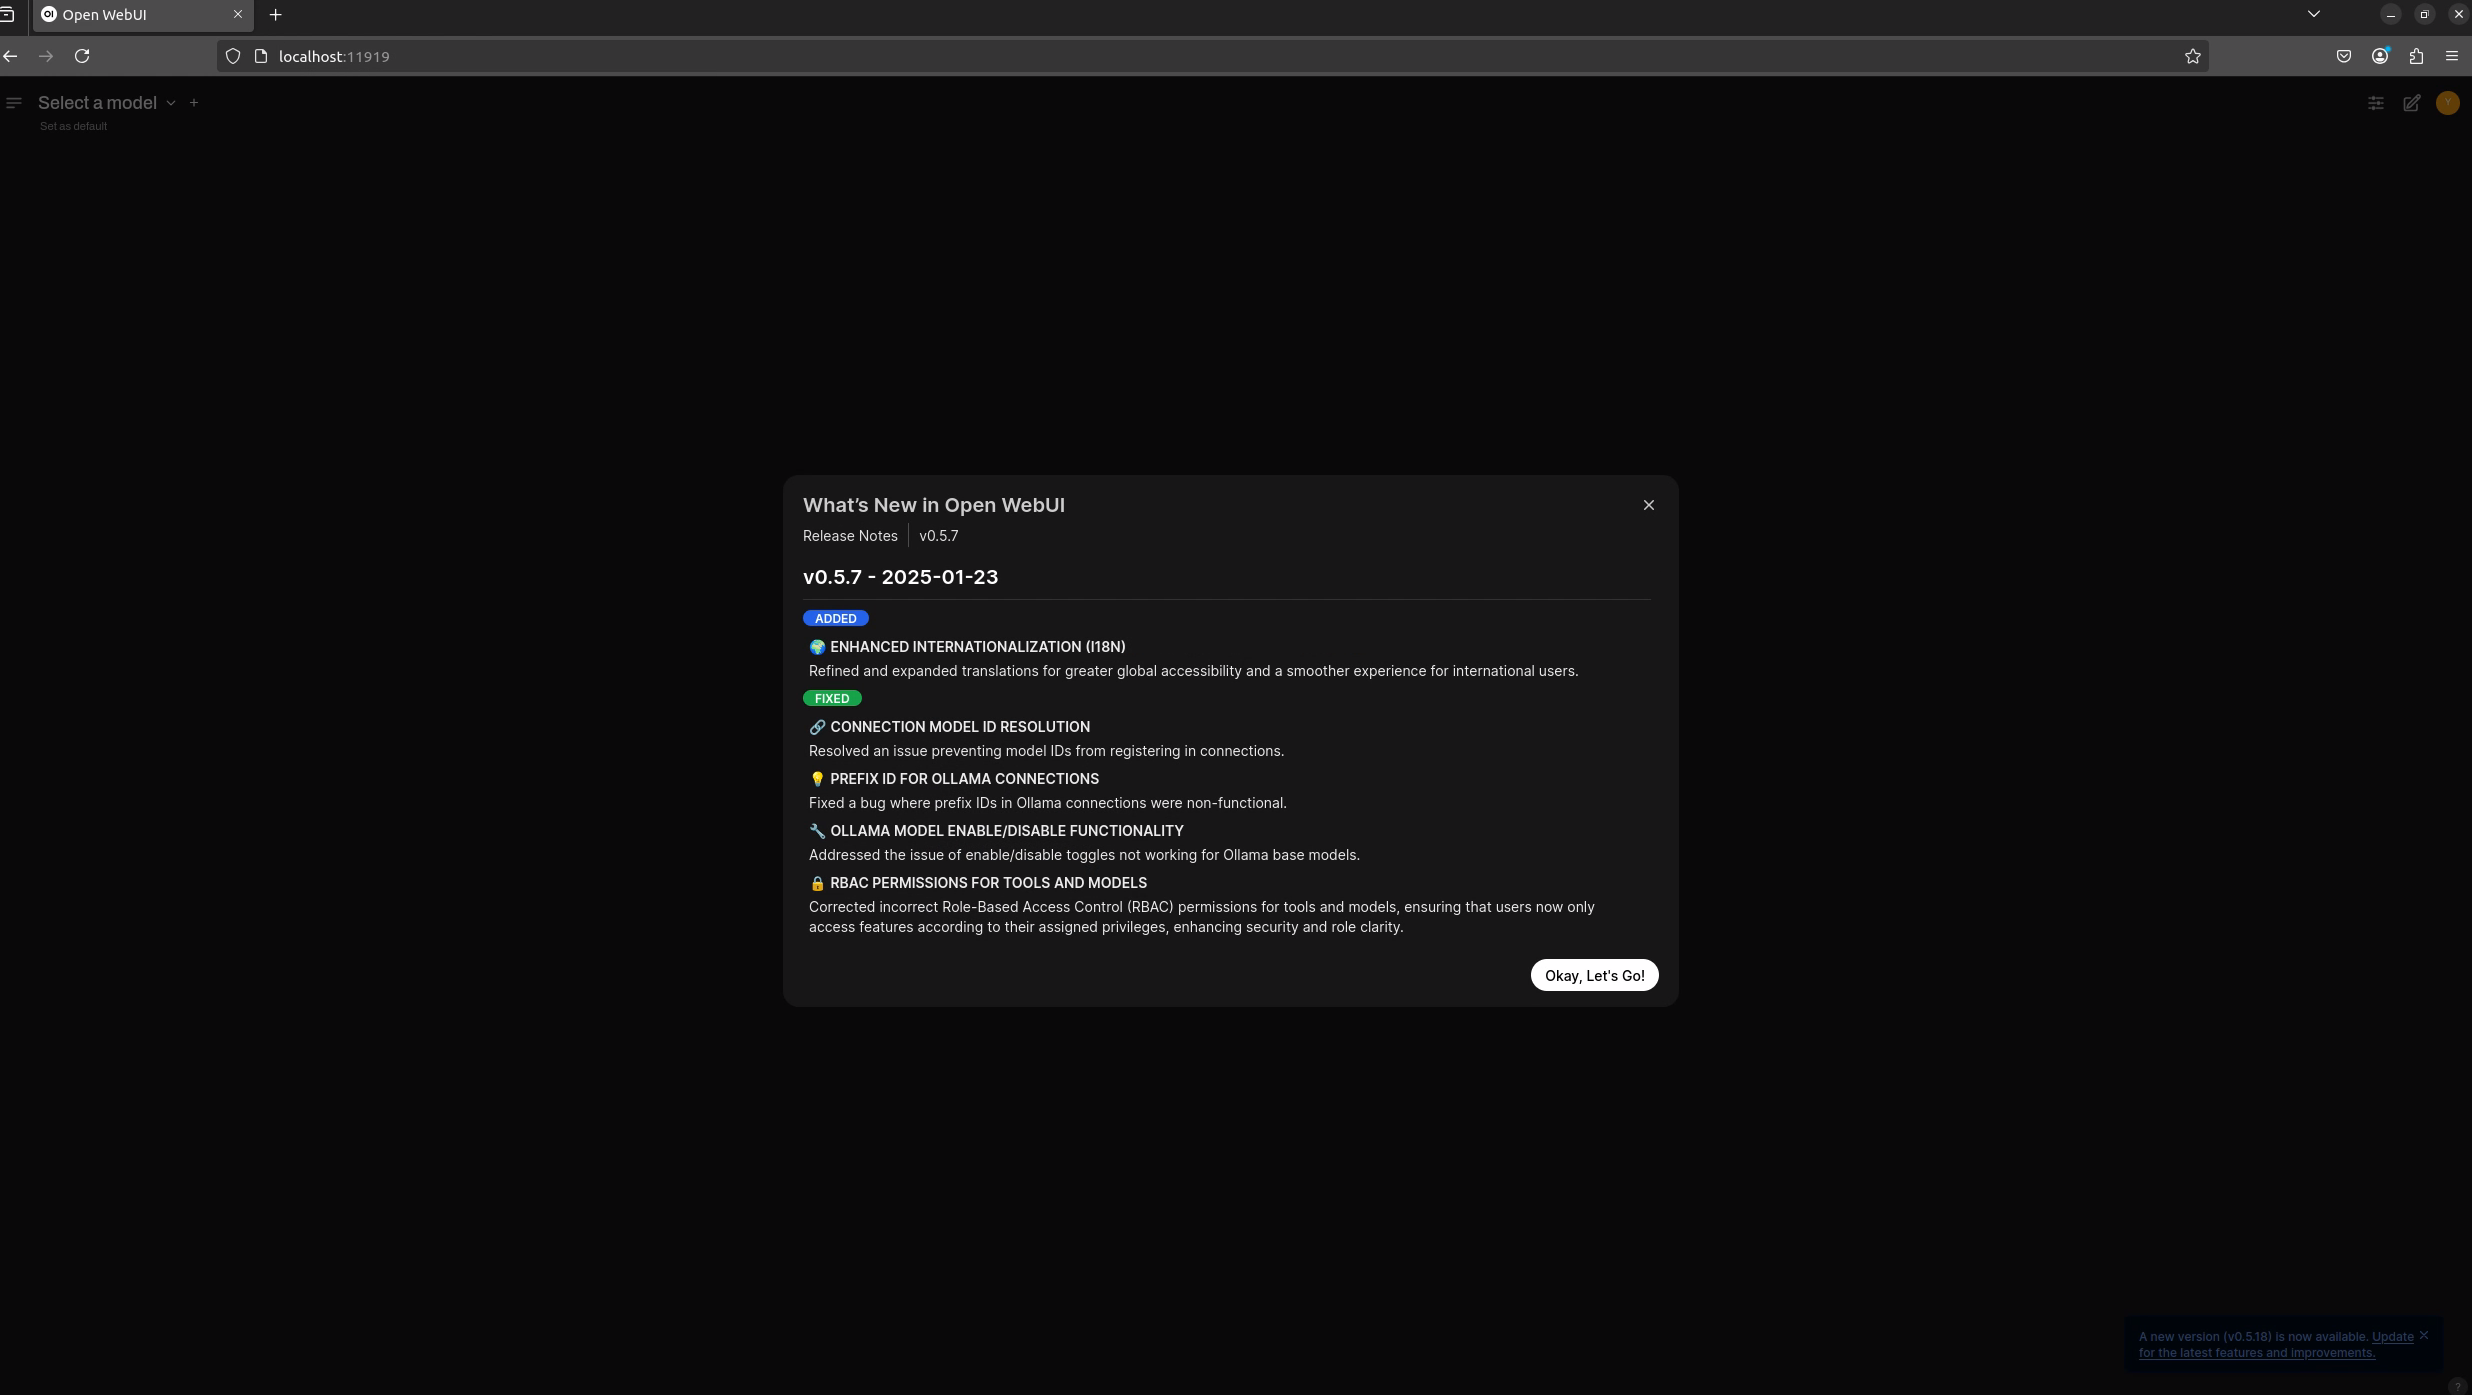
\includegraphics[width=0.8\linewidth]{images/Pasted image 20250304171722.png}
\end{figure}

この時点では,モデルリストは空である.

\begin{figure}[H]
    \centering
    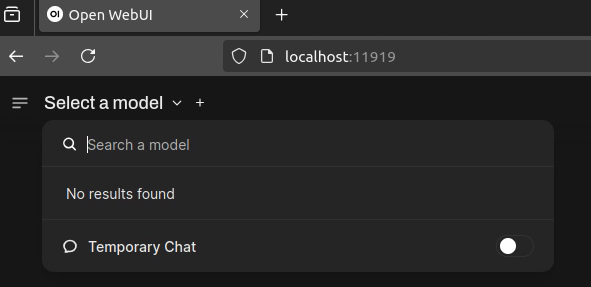
\includegraphics[width=0.8\linewidth]{images/Pasted image 20250304171753.png}
\end{figure}

\paragraph{注意} 長時間GPUを使用しない場合,NVIDIAのドライバがGPUとの接続を自動で切断し,推論速度が大幅に低下する場合がある(CPU推論に切り替わる).その際は,以下のコマンドでコンテナを再起動すること.
\begin{lstlisting}[language=bash]
docker restart open-webui-ollama
\end{lstlisting}

\section{ローカルデプロイしたOpen WebUI(Local Deployment)の使用方法}
LLMとの対話には,まず\href{https://ollama.com/search}{Ollamaサポートモデル一覧}から適切なモデルを選択する.例えば「deepseek-r1」シリーズを使用する場合,ウェブページで異なるパラメータサイズのGPU MEM使用量を確認し,自身の環境に合ったモデルを選択する.もし「deepseek-r1:14b」モデルを使用する場合は以下のコマンドを実行する:

\begin{lstlisting}[language=bash]
docker exec -it open-webui-ollama ollama run deepseek-r1:14b
\end{lstlisting}

\paragraph{コマンドパラメータ解説}
\begin{itemize}
\item \texttt{exec}: コンテナ内でコマンドを実行.コンテナ内で特定のコマンドを実行するためのサブコマンド.
\item \texttt{-it}: インタラクティブモード.リアルタイムのダウンロード進捗表示と対話型インタフェースを有効化.
\item \texttt{open-webui-ollama}: 対象コンテナ名の指定.デプロイ時に設定したコンテナ名と一致させる必要がある.
\item \texttt{ollama run deepseek-r1:14b}: コンテナ環境内で実行するコマンド.モデルのダウンロードと実行を同時に実施.
\end{itemize}

このコマンドにより「deepseek-r1:14b」モデルが自動的にダウンロードされる.コマンドラインでの対話例:
\begin{lstlisting}[language=bash]
% docker exec -it open-webui-ollama ollama run deepseek-r1:14b
>>> How do you do?
<think>

</think>

Hi! I'm DeepSeek-R1, an artificial intelligence assistant created by
DeepSeek. For comprehensive details about our models and products, we
invite you to consult our official documentation.

>>> /bye
\end{lstlisting}

いま\texttt{http://localhost:11919} にアクセスすると,下のような画面が表示される.

\begin{figure}[H]
    \centering
    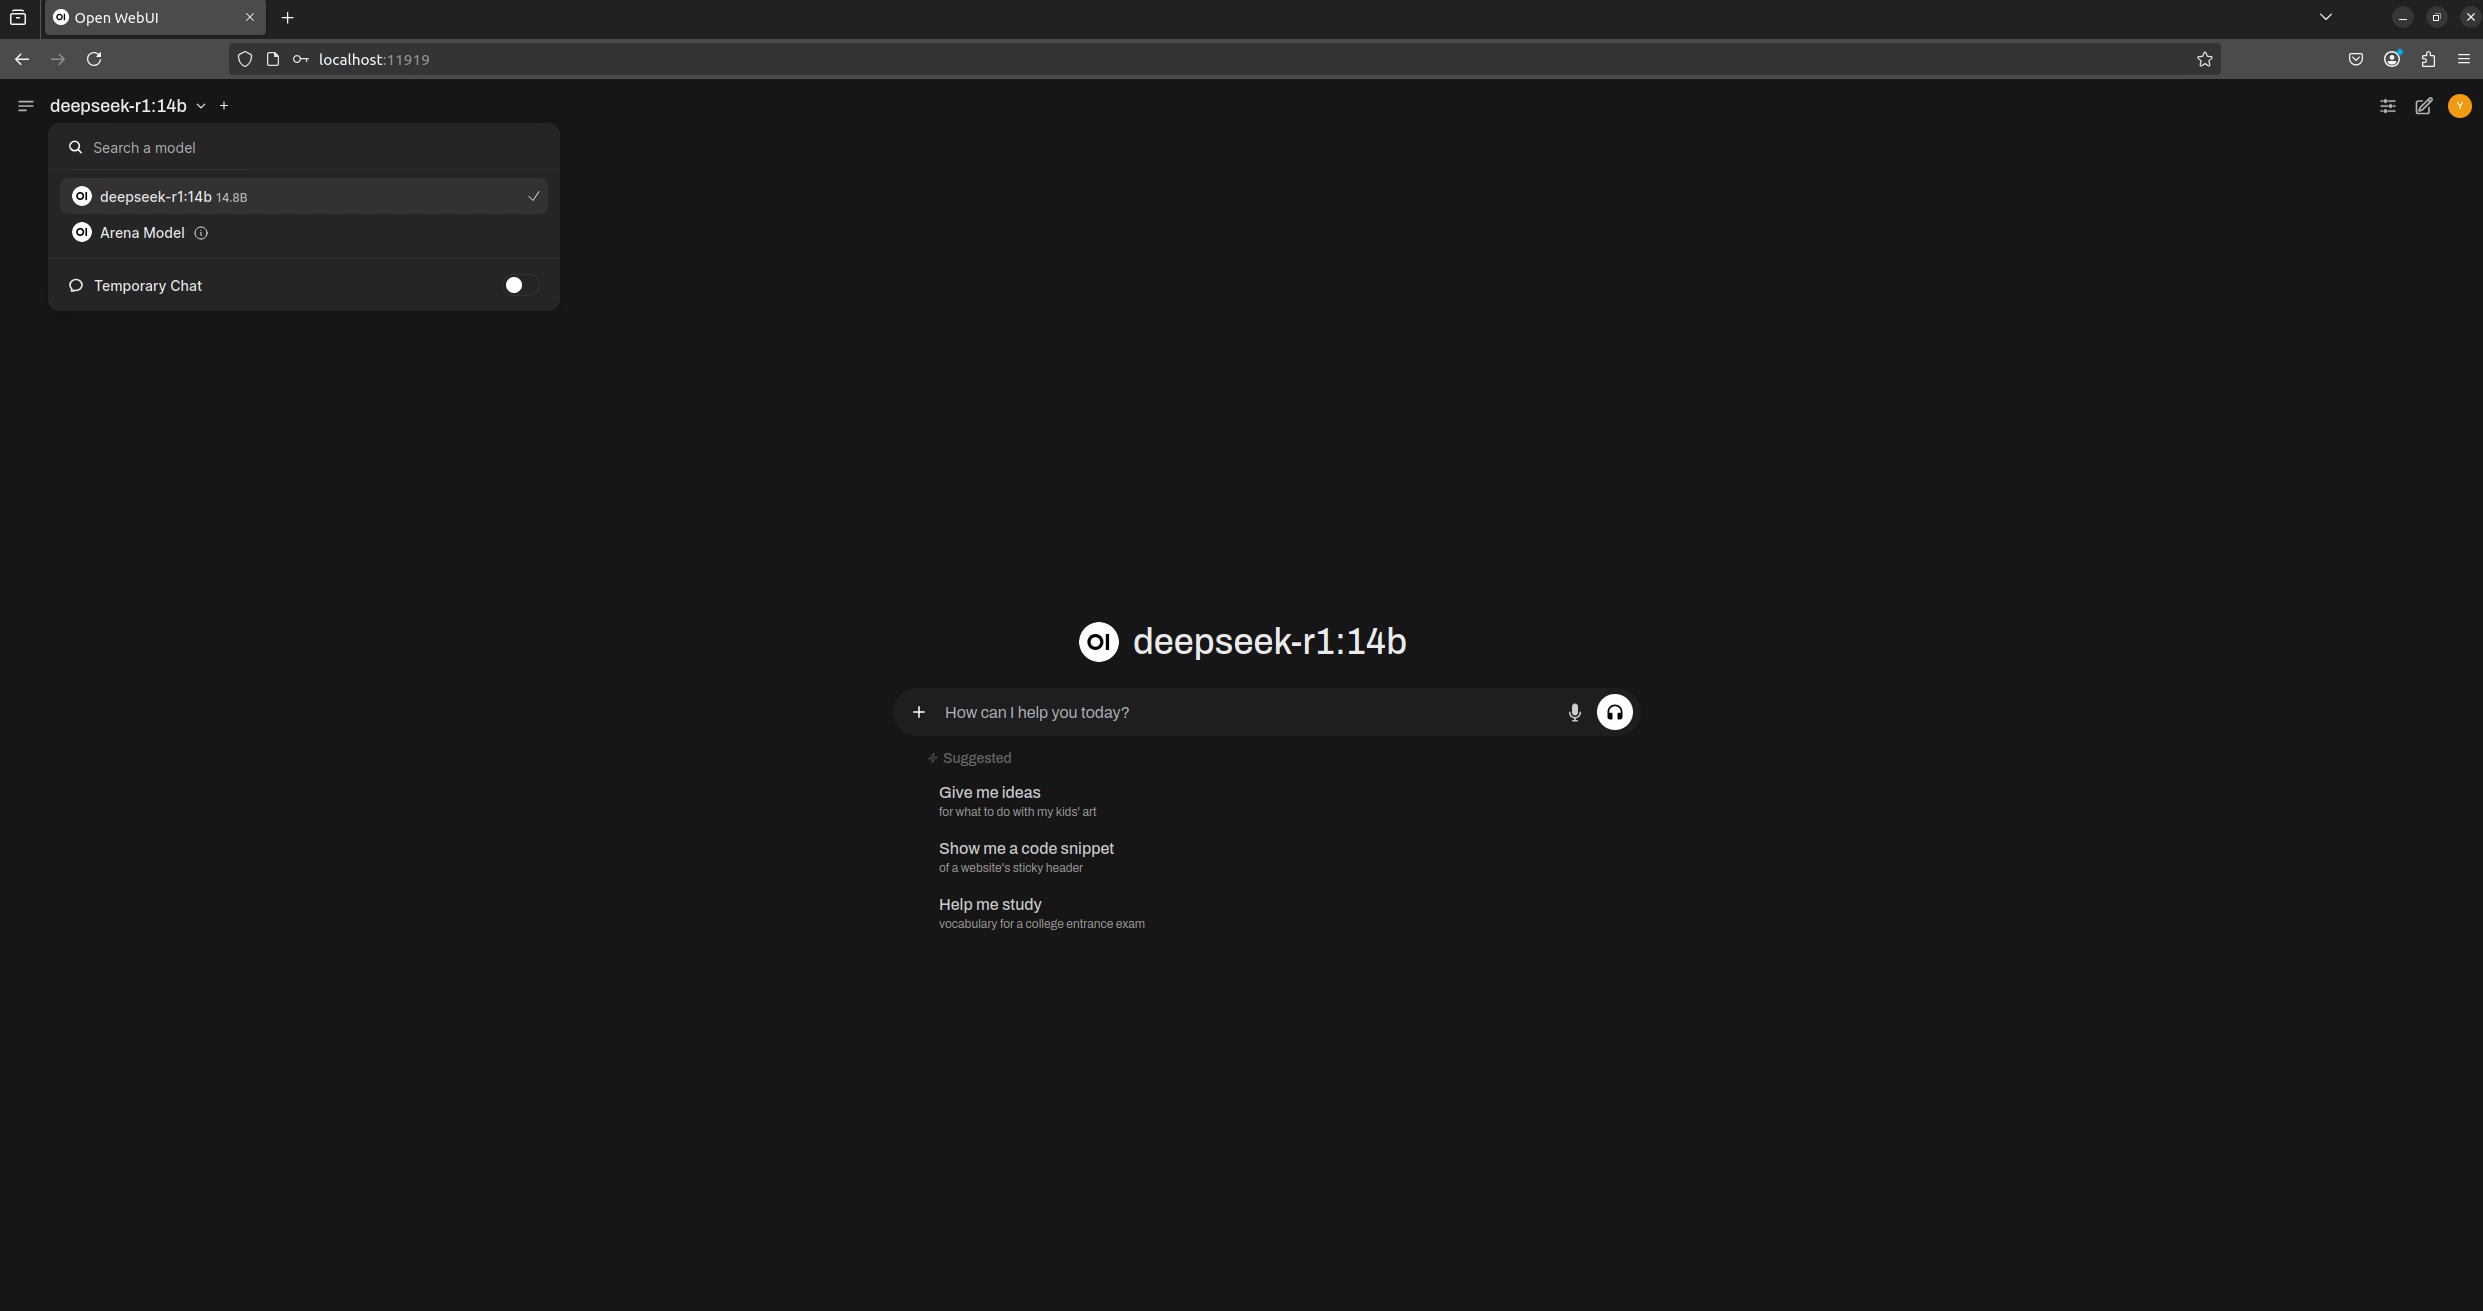
\includegraphics[width=0.8\linewidth]{images/Pasted image 20250304170628.png}
\end{figure}

\paragraph{高度な設定}
右上のモデルパラメータ設定では以下の調整ができる:
\begin{itemize}
\item 温度(Temperature): 生成テキストのランダム性を制御.
\item 最大トークン数(Max Tokens): 生成テキストの長さを制限.
\item トップP(Top-P): 確率分布に基づくサンプリング範囲を調整.
\end{itemize}

その他の機能(ユーザ権限管理,ネットワーク検索サービス連携等)は設定メニューで確認できる.詳細な機能探索はユーザ自身で活用してください.

\paragraph{技術的注意点}
\begin{itemize}
\item 「docker exec」コマンド実行前に対象コンテナ(open-webui-ollama)が正常に起動していることが必要.
\item 「ollama run」コマンドはモデル未ダウンロード時に自動取得するが,1-30分程度要する場合がある(ネットワーク速度に依存).
\item モデルダウンロードにはGPU MEMとディスク容量が十分にあることを確認すること.メモリ不足時はより小さいモデル(例:7B)の選択を推奨.
\end{itemize}